\chapter{Introduction}\label{cha:introduction}
This document is a pilot's manual for XCSoar, an open-source glide
computer originally developed for Pocket PC devices.  The audience 
is assumed to have a sound knowledge of the fundamental theory of flight for
gliders, and at least a basic working knowledge of cross-country soaring.

Updates to the XCSoar software may result in some of this manual being
out of date. You should read the release notes distributed with the
software to keep track of changes.  Updates to the manual and software
are available from 
\begin{quote}
\xcsoarwebsite{}
\end{quote}

\section{Organization of this manual}

\todonum[inline]{Write about the manual crossref hinting icons and the yellow
colour. The Quickstart will be readable also without those links available} 
This manual most notably is written in order to get the XCSoar user started 
quickly  \emph{as well as} support his deep understanding of all the features, 
concepts and tactics introduced. At all times, the authors made their effort 
for doing this from a pilot's perspective (and honestly hope for having 
succeeded).

The authors highly encourage you to take your time reading the entire manual 
chapter by chapter (with exception of the reference chapters Infoboxes and 
Configuration). Feel assured, the time you will have spent will pay off as a 
manifold in understanding. On your way reading you might feel blue once in a 
while. That is why the authors introduced some blueish things: links and 
icons.

\begin{figure}[h]
\centering

\includegraphics[width=0.8cm,angle=0,keepaspectratio='true']{figures/config.pdf}
\hspace{1.5cm}
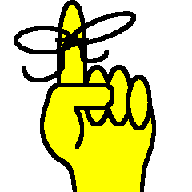
\includegraphics[width=0.8cm,angle=0,keepaspectratio='true']{figures/reminder.pdf}
\hspace{1.5cm}

\includegraphics[width=0.8cm,angle=0,keepaspectratio='true']{figures/gesture.pdf}
\hspace{1.5cm}

\includegraphics[width=0.8cm,angle=0,keepaspectratio='true']{figures/warning.pdf}
\caption{Icons configuration, reminder, gesture, warning}
\end{figure}

\warning Warning. The icon warning is used, whenever things shall be followed 
strictly.  Not following will cause unexpected results, total dysfunction, or
even danger to life. Proceed only, if warning understood.

\gesture{DU} Gesture. A swipe gesture input is available using devices with a 
touch screen to invoke a menu or function amongst others. In this example, DU 
stands for moving your fingertip down, then up, (in straight lines) on the 
screen.
  
\gesturespec{du} Specific Gesture. Whenever the manual's authors kept up with XCSoar's rapid development process
in writing, a specific icon is provided, depicting the movements.

\tip Reminder. This icon tags a tip, trick, things you might remind after having read corresponding sections and so on.

\config{orientation} Configuration see... The icon depicting two craftsman's
tools refers to an in-depth description of items being mentioned and how to 
configure them. The numbers beside the icon refer to a specific chapter / 
section of this manual's reference chapters \ref{cha:infobox} and 
\ref{cha:configuration}, in this case referring to section 
\ref{conf:orientation}. 

\marginlabel{\parbox{1.3cm}{\rotatebox[origin=c]{180}{
\includegraphics[width=0.9cm]{figures/warning.pdf}}}}
\rotatebox[origin=c]{180}{Stop from reading manuals whilst flying inverted!}

\emph{Read} at home, \emph{configure} on the ground, safely. Having perceived 
this (inverted) warning as an example, you are ready to proceed.

\config{usingxcsoarsafely} Referring to the second exemplary case of the icon 
``configuration'' to the left, the icon points
towards chapter \ref{cha:introduction}, (this chapter), section 
\ref{sec:usingxcsoarsafely}, ``Using XCSoar safely'' underneath, which could be
understood as a ``how to configure yourself''. It is up to you whether to jump
to an in depth discussion and go back or just proceed. If reading this manual 
electronically, clicking the number will let you jump to the requested cross
-reference.  Use the go-to ``back'' (or similar) function of your particular
browser to proceed with the chapter you jumped from.

The numbers are printed in blue as are the icons introduced, signalling ``help
available''. And so are other Universal Resource Locators, underlying blue
text. Clicking on text like \xcsoarwebsite{/contact} will open your world wide 
web browser or mailer to get in touch with other resources or knowledgeable
people respectively.

The remainder of this chapter ``Introduction'' is about getting you prepared for
XCSoar, how to raise your level of understanding and maintain your skills. 
Chapter \ref{cha:quickstart} ``Quickstart'' might be the next waypoint after
\ref{cha:installation} ``Installation'' for the urgent user. Feel free to cut
short, but do not resume too sadly when reading chapter by chapter, following:

Chapter~\ref{cha:interface} introduces the user interface
concepts and gives an overview of the display .

Chapter~\ref{cha:navigation} describes the moving map part of the
display in greater detail and describes how the software can assist in
general navigation.  Chapter~\ref{cha:tasks} describes how
cross-country tasks are specified and flown, and presents some of the
analysis tools available to pilots to help improve their performance.
Chapter~\ref{cha:glide} goes into further detail on the glide computer
functions as it is important for pilots to be aware of how the
computer performs its calculations.

Chapter~\ref{cha:atmosph} describes how the computer can interface to
variometers and other air data sensors, and how it uses these
measurements to provide various models of the atmosphere, in
particular on winds and thermal convection.
Chapter~\ref{cha:airspace} describes how XCSoar can assist in managing
flight in special use airspace and the FLARM collision awareness
system.  Chapter~\ref{cha:avionics-airframe} deals with systems
integration and systems diagnostics, the integration of XCSoar with
communications devices and with airframe switches.

The remainder of the manual contains mainly reference material.
Chapter~\ref{cha:infobox} lists the types of information that can be
displayed in the grid of InfoBoxes next to the map display.  The
configuration of the software is described in detail in
Chapter~\ref{cha:configuration}.  The formats of the various data
files that program uses, as well as where to obtain them from and how
to edit them, is described in Chapter~\ref{cha:data-files}.

Finally, a short history and discussion of XCSoar's development
process is presented in Chapter~\ref{cha:history-development}.

\section{Notes}

\subsection*{Screenshots}
Throughout this manual are several screenshots of XCSoar. These are
taken from the program running on a variety of hardware platforms and possibly
even different versions. Each platform and version may have different screen
resolutions, layouts and fonts, and so there may be slight differences in the
appearance of the display. Most of the screenshots in this manual are taken of
XCSoar running in landscape orientation.

\section{Platforms}
\begin{description}
\item[Android Devices]
XCSoar runs on Android 1.6 or newer.
\item [eBookreader]
XCSoar runs on some Kobo eReader devices. A native port has been released with version 6.7.1, but is still considered experimental (Nov. 2013).
\item[Windows PC]
It is possible to run XCSoar on an ordinary computer with the Windows
operating system. This setup can be used for training yourself in using XCSoar.
A simulation mode is included in XCSoar as well as a IGC replay function, that
can be used when not connected to a valid GPS source.
\item[Unix/Linux PC]
XCSoar can be run on Unix using the Wine emulator. A native Unix port
has been released with the 6.0 version of XCSoar, but is still
considered experimental.
\end{description}



\section{Technical support}

\subsection*{Troubleshooting}
A small team of dedicated developers produces XCSoar. Although we are
happy to help with the use of our software, we cannot teach you about
basics of modern information technology. If you have a question about XCSoar in
particular not found in this manual please get in touch. You will find all of the following links summarized at:
\begin{quote}
\xcsoarwebsite{/contact}
\end{quote}
To begin with communication, join the XCSoar forum at:
\begin{quote}
\url{http://forum.xcsoar.org}
\end{quote}
If your concern appears not already addressed, post it or email us: 
\begin{quote}
\href{mailto:xcsoar-user@lists.sourceforge.net}{xcsoar-user@lists.sourceforge.net}
\end{quote}
Any frequent questions will be added to this document and to the Frequently
Asked Questions (FAQ) section of the XCSoar website.
You may also find it useful to subscribe to the XCSoar users mailing
list so you will be kept up to date with latest developments.

If all of this does not help, you probably discovered a bug.

\subsection*{Feedback}
Like any complex software program, XCSoar may be subject to software
bugs, so if you find any, please report them to the XCSoar developers
by using our bug tracker portal at: 
\begin{quote}
\xcsoarwebsite{/trac}
\end{quote}
or by sending an email to
\begin{quote}
\href{mailto:xcsoar-devel@lists.sourceforge.net}{xcsoar-devel@lists.sourceforge.net}
\end{quote}
XCSoar logs many valuable things in a logfile
\verb|xcsoar.log| in the \texttt{XCSoarData} directory. The logfile can be appended to the bug ticket in order to help XCSoar developers determine the cause of possible problems.
If you like the idea of doing some more, get involved:
\begin{quote}
\xcsoarwebsite{/develop}
\end{quote}

\subsection*{Updates}
You should periodically visit the XCSoar website to check for program
updates. The installation procedure described above can typically be
repeated in order to upgrade the software.  All user configuration
settings and data files will be preserved during the
re-installation/upgrade.

It is also recommended to periodically check for updates to data
files, particularly Special Use Airspace, which may be subject to
change by the national civil aviation authority.

\section{Training}
For the safety of yourself and others, pilots using XCSoar are advised to
train themselves in using XCSoar on the ground and become familiar with its
interface and features prior to flight.

\subsection*{Using XCSoar on the PC}
The PC versions of XCSoar may be used to become familiar with XCSoar's
interface and functionality in the comfort of one's home.  All files
and configuration used by this version are identical to the embedded versions,
so it can be helpful to try out customisations on the PC version before using
them in flight.

The PC versions can also be connected to external devices and operate just as
the embedded versions do. Suggested uses include:
\begin{itemize}
\item Connect the PC to a FLARM device to use XCSoar as a ground
station display of FLARM-equipped traffic.
\item Connect the PC to an intelligent variometer such as Vega to
test configuration settings of the variometer.
\end{itemize}

\subsection*{Using XCSoar with a flight simulator}
A good way to learn how to use XCSoar is to connect the Pocket PC
device to a PC running a flight simulator that can output NMEA
sentences to the serial port. Suitable simulators include Condor and
X-Plane.  

The benefit of this form of training is that XCSoar can be used in FLY
mode, so it behaves exactly as if you were really flying, and you can
get a good feel for how the program works while you are flying the
simulator.

\section{Using XCSoar safely}\label{sec:usingxcsoarsafely}\label{conf:usingxcsoarsafely}
The use of an interactive system like XCSoar in flight carries with it
certain risks due to the potential distraction of the pilot from
maintaining situational awareness and eyes outside the cockpit.

The philosophy guiding the design and development of the software is
to try to reduce this distraction by minimising the need for user
interactions as much as possible, and by presenting information in a
clear fashion able to be interpreted at a glance.

Pilots using XCSoar must take responsibility for using the system safely.
Good practice in the use of XCSoar includes:
\begin{itemize}
\item Becoming familiar with the system thoroughly through training on 
  the ground.
\item Performing clearing turns before interacting with XCSoar in flight
  in order to ensure there is no collision risk with other traffic.
\item Setting up the system to take advantage of automatic functions
  and input events so that user interactions can be minimised.  If you
  find yourself mechanically performing certain interactions frequently,
  ask yourself (or other XCSoar users) if the software can be made to do 
  these interactions for you.
\end{itemize}
